\section{Details of Environments and Implementation}

\begin{figure}[h!]
  \begin{center}
    \subfloat[Predator and prey (PP)]
    {\label{fig:pp}
      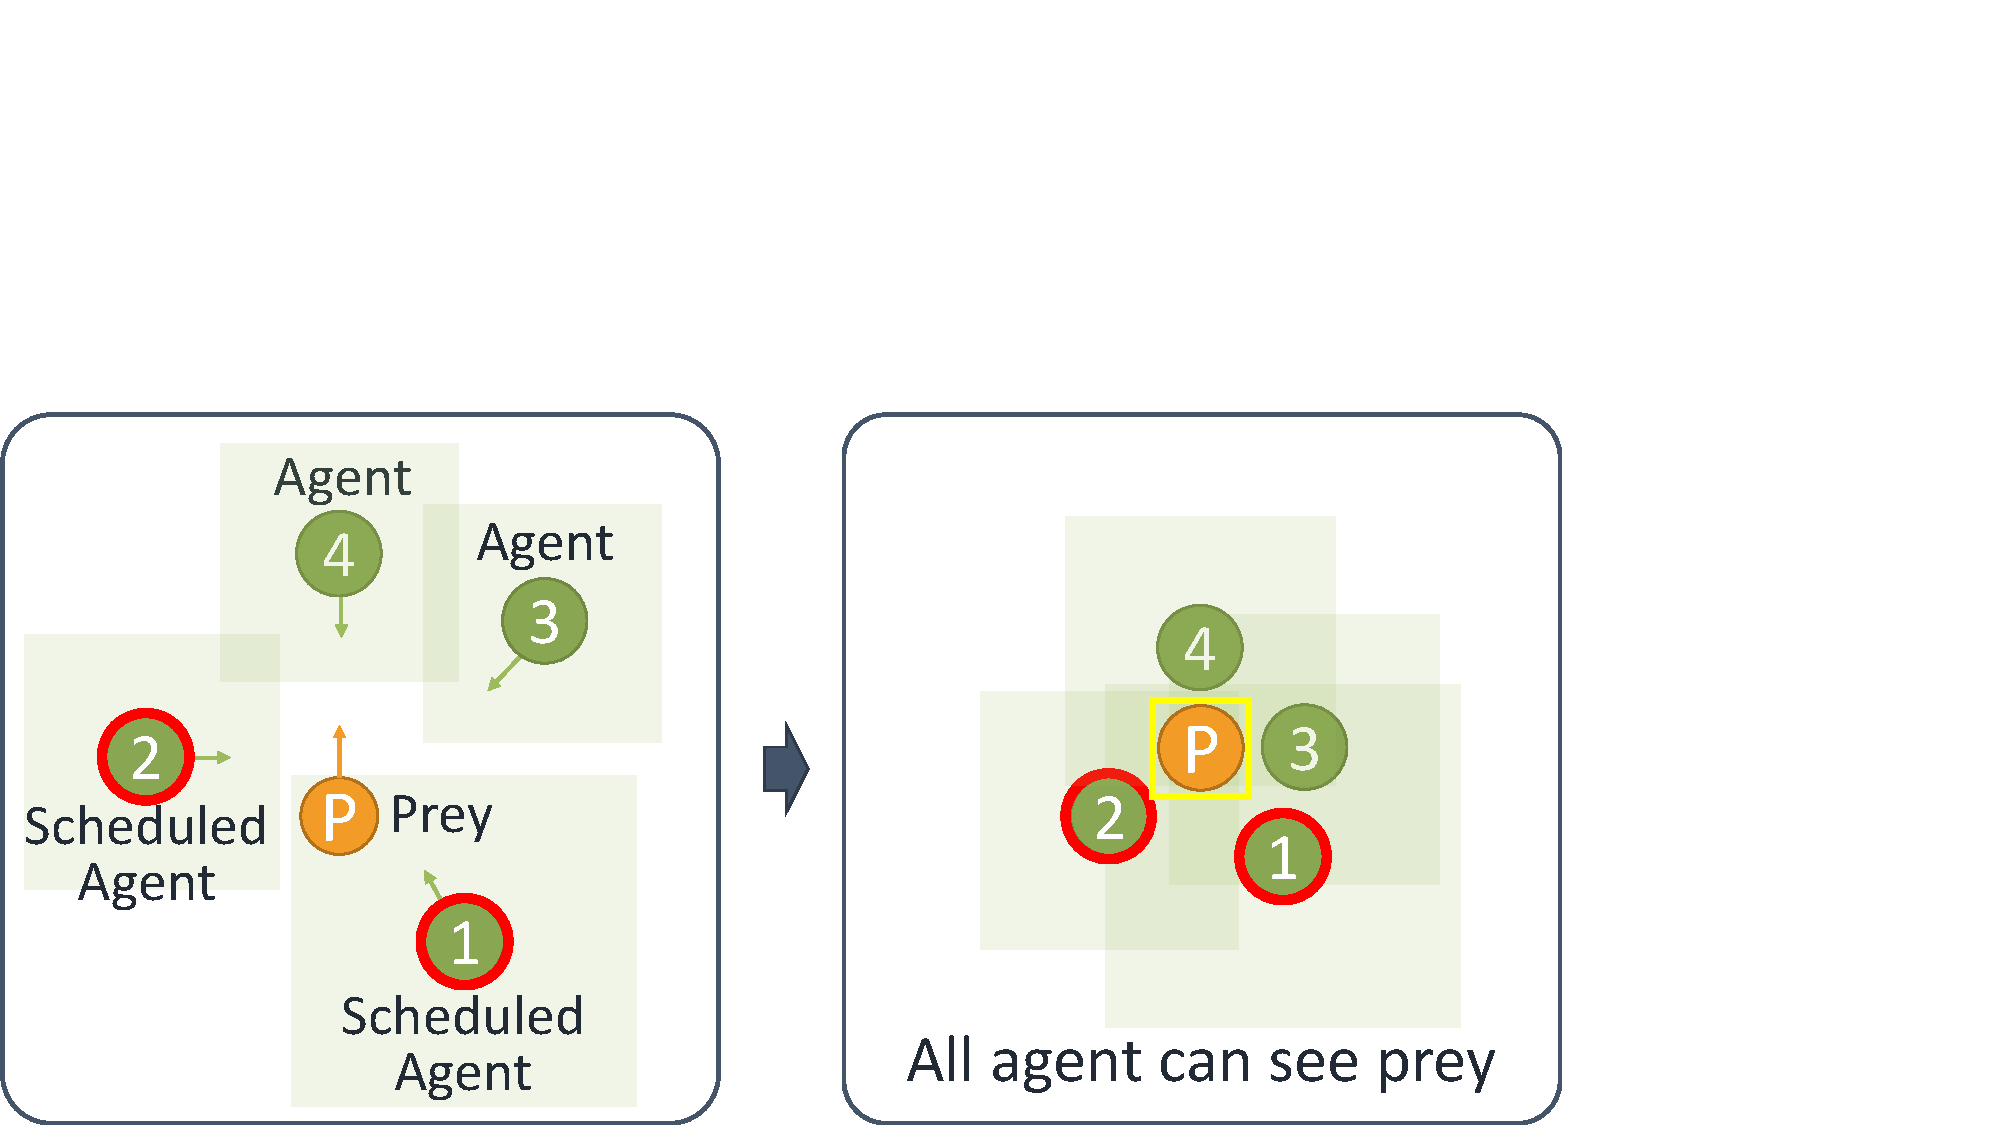
\includegraphics[width=0.40\columnwidth]{fig7} }
    \hspace{0.7cm}
    \subfloat[Cooperative communication and navigation (CCN)] {\label{fig:ccn}
      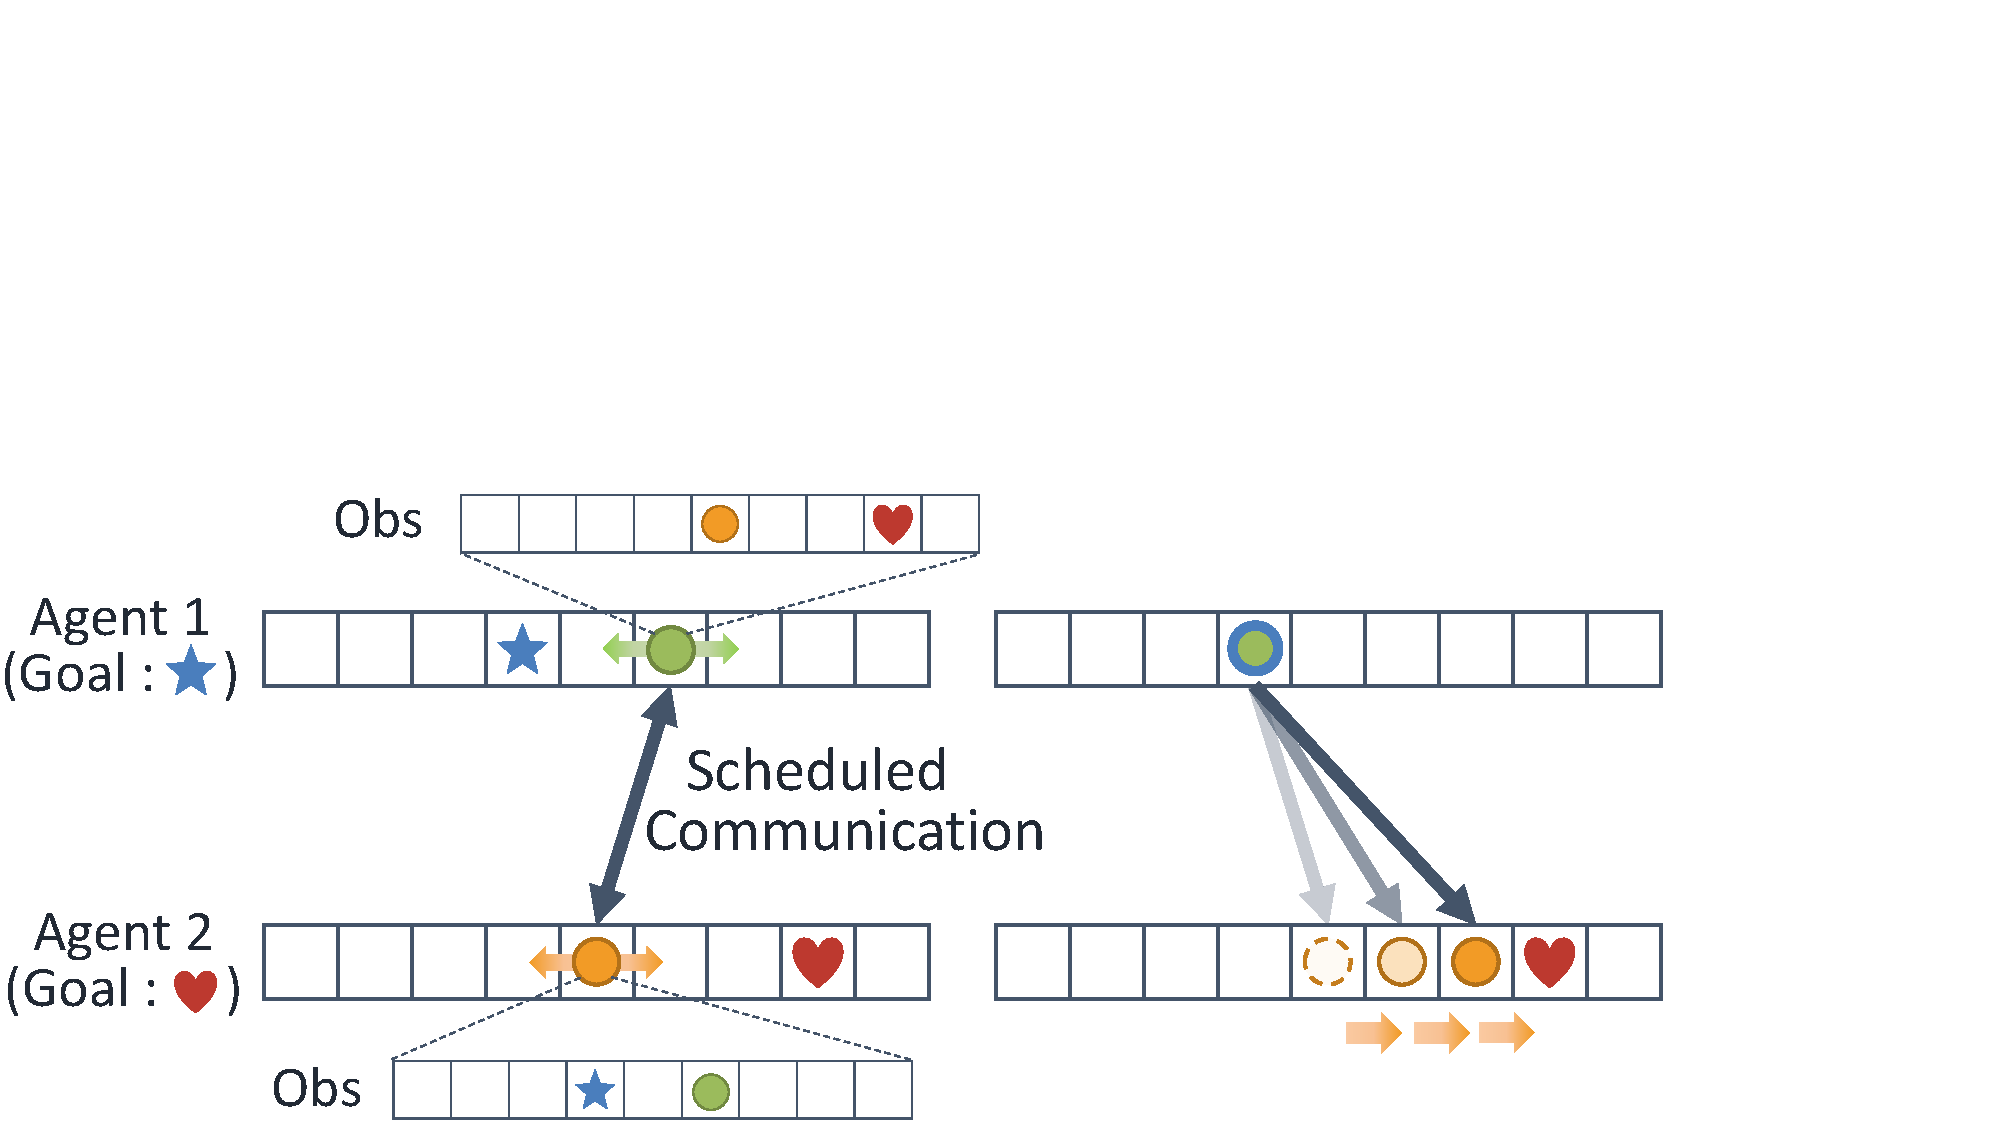
\includegraphics[width=0.44\columnwidth]{fig8} }
  \end{center}
  \vspace{-0.2cm}
  \caption{Illustrations of the experimental environment}
  \label{fig:scenario}
\end{figure}


\subsection{Environments: PP and CCN}

\myparagraph{Predator and prey}
We assess \sched~in this predator-prey setting as in
\cite{stone2000multiagent}, illustrated in Figure \ref{fig:pp}.  This
setting involves a discretized grid world and multiple cooperating
predators who must capture a randomly moving prey. Agents'
observations include position of themselves and the relative positions
of the prey, if observed. The observation horizon of each predator is
limited, thereby emphasizing the need for communication. The
termination criterion for the task is that all agents observe the
prey, as in the right of Figure~\ref{fig:pp}. The predators are
rewarded when the task is terminated.
% \note{The global system state fed into the critic network is encoded as a concatenated list of
% coordinates of each agents to mitigate the curse of dimensionality
% when growing the size of the map. }
% The current self-position of each agent
% is also embedded into the observation vector at each time step.
We note that agents may be endowed with
different observation horizons, making them heterogeneous. 
We employ four agents in our experiment, where only agent 1 has a $5 \times 5$ view
while agents 2, 3, and 4 have a smaller, $3 \times 3$ view.
The performance metric is the number of time steps taken to capture the prey.

\paragraph{Cooperative communication and navigation}
We adopt and modify the cooperative communication and navigation task
in \cite{lowe2017multi}, where we test \sched~in a simple
one-dimensional grid as in Figure~\ref{fig:ccn}. In CCN, each of the two
agents resides in its one-dimensional grid world. Each agent's goal is
to arrive at a pre-specified destination (denoted by the square with a
star or a heart for Agents 1 and 2, respectively), and they collect a
joint reward when both agents reach their target destination. Each
agent has a zero observation horizon around itself, but it can observe
the situation of the other agent. We introduce heterogeneity into the
scenario, where the agent-destination distance at the beginning of the
task differs across agents.
In our example, Agent 2 is initially located at a farther place from
its destination, as illustrated in Figure~\ref{fig:ccn}. The metric
used to gauge the performance of \sched~is the number of time steps
taken to complete the CCN task.


\subsection{Experiment Details}
Table~\ref{table:hyperparameter} shows the values of the hyperparameters for the CCN and the PP task. 
We use Adam optimizer to update network parameters and soft target update to update target network. The structure of the networks is the same across tasks.
For the critic, we used three hidden layers, and the critic between the scheduler and the action selector shares the first two layers. For the actor, we use one hidden layer; for the encoder and the weight generator, three hidden layers each. Networks use rectified linear units for all hidden layers.
Because the complexity of the two tasks differ, we sized the hidden layers differently. The actor network and the critic network for the CCN have hidden layers
with 8 units and 16 units, respectively. The actor network and the critic network for the PP have hidden layers with 32 units and 64 units, respectively.


\begin{table}[h!]
  \centering
  \caption{\small List of hyperparameters}
  \label{table:hyperparameter}
  \begin{tabular}{@{}lllll@{}}
  \toprule
  \textbf{Hyperparameter}       & \textbf{Value} & \multicolumn{3}{l}{\textbf{Description}}                                \\ \midrule
  training step                 & 750000         & \multicolumn{3}{l}{Maximum time steps until the end of training}        \\
  episode length                & 1000            & \multicolumn{3}{l}{Maximum time steps per episode}                      \\
  discount factor               & 0.9            & \multicolumn{3}{l}{Importance of future rewards}                        \\
  learning rate for actor       & 0.00001        & \multicolumn{3}{l}{Actor network learning rate used by Adam optimizer}  \\
  learning rate for critic      & 0.0001         & \multicolumn{3}{l}{Critic network learning rate used by Adam optimizer} \\
  target update rate            & 0.05           & \multicolumn{3}{l}{Target network update rate to track learned network} \\
  entropy regularization weight & 0.01           & \multicolumn{3}{l}{Weight of regularization to encourage exploration}   \\
  \bottomrule
  \end{tabular}
  \end{table}



%%% Local Variables:
%%% mode: latex
%%% TeX-master: "main"
%%% End:
